\documentclass[twoside,11pt]{article}

% Any additional packages needed should be included after jmlr2e.
% Note that jmlr2e.sty includes epsfig, amssymb, natbib and graphicx,
% and defines many common macros, such as 'proof' and 'example'.
%
% It also sets the bibliographystyle to plainnat; for more information on
% natbib citation styles, see the natbib documentation, a copy of which
% is archived at http://www.jmlr.org/format/natbib.pdf

\usepackage{jmlr2e}
\usepackage{setspace}

% Graphics
\usepackage{graphicx}
\graphicspath{ {images/}}

% Definitions of handy macros can go here
\newcommand{\dataset}{{\cal D}}
\newcommand{\fracpartial}[2]{\frac{\partial #1}{\partial  #2}}

% Heading arguments are {volume}{year}{pages}{date submitted}{date published}{paper id}{author-full-names}

\jmlrheading{1}{2000}{1-48}{4/00}{10/00}{meila00a}{Christopher Jeschke}

% Short headings should be running head and authors last names

\ShortHeadings{Dissertation Critique}{Jeschke}
\firstpageno{1}

\begin{document}

\title{Dissertation Critique: Exploring Machine Learning Techniques Using Patient
      Interactions In Online Health Forums to Classify Drug Safety}

\author{\name Christopher Jeschke \email cjeschk2@jhu.edu \\
       \addr Engineering for Professionals\\
       Johns Hopkins University\\
       Elkridge, MD 20175, USA}

\editor{n/a}

\maketitle


% Entire paper should be single spaced
\singlespacing

% Abstract
\begin{abstract}%   <- trailing '%' for backward compatibility of .sty file
  Patient generated health data represents an area of active research interest
  for its potential applications in improving the public health. The study of
  Pharmacovigilance is one such area, focused on monitoring drugs once they have been
  released to market. Dr. Brant Chee's 2011 dissertation applying machine learning
  techniques to patient messages in online health forums explores how watch
  list drugs from the United States Food and Drug Administration can be detected
  via these forum messages, ultimately with the intent to alert consumers to drug
  safety concerns.
\end{abstract}

\begin{keywords}
  Drug Safety, Pharmacovigilance, NLP
\end{keywords}


\section{Summary of Research}
%Todo:  Fix Niave Bayes double dot
Dr. Brant Chee's 2011 dissertation \textit{Exploring Machine Learning Techniques Using
Patient Interactions in Online Health Forums to Classify Drug Safety} describes
Chee's research in applying natural language processing (NLP) techniques in conjunction with Naive Bayes and Support Vector Machine classifiers to identify candidate \textit{watch list} drugs from online patient forums. Watch list drugs are those drugs identified by the United States Food and Drug Administration (FDA) as presenting a significant health or safety risk to drug consumers, thereby prompting regulatory action to better inform the consumer or directly protect the consumer by removing the drug from market or reducing its accessibility. Chee's dissertation seeks to answer the specific questions:
\begin{itemize}
  \item Can Machine Learning classification methods using text features extracted from online health forums be used to identify FDA watch list drugs?
  \item Is the sentiment of the forum message useful in identifying these drugs?
  \item Similarly, are the drug effect entities useful in identifying watchlist drugs?
\end{itemize}

This research is accomplished through an empirical study using a corpus from the
Yahoo! public health forums, against which Chee applies various NLP techniques
to define and distill a feature space for classification using Niave Bayes and
Support Vector machines for detecting watchlist drugs. Drugs detected are
evaluated against watchlist drugs found via the FDA Adverse Event Reporting System (AERS) to determine the utility of the approach and its applicability in Pharmacovigilance.

\subsection{Background on Pharmacovigilance, AERS and Social Media}
The dissertation begins with an extensive background discussion on adverse drug reactions and current surveillance techniques. Adverse drug reactions are defined by the FDA and World Health Organization (WHO) as "A response to a drug which is noxious and unintended and which occurs at doses normally used in man for prophylaxis, diagnosis, or therapy of disease or for modification of physiological function."\cite{FDA}. Chee continues by introducing Pharmacovigilance as "the study of drugs once released to market"\citp{Chee}, and the important regulatory agencies practicing it are mentioned - the World Health Organization (WHO) and United States Food and FDA. The FDA Adverse Event Reporting system (AERS) is discussed as comparison with it is central to the work. AERS was constructed to house mandatory drug safety reports from drug manufacturers, distributors and health care facilities, as well as voluntary reports submitted by consumers (patients), physicians and other healthcare providers. Reports are evaluated by the Center for Drug Evaluation and Research (CDER) and Center for Biologics Evaluation and Research (CBER) within the FDA for drug safety signals, which may then be elevated for further review by clinicians, epidemiologists and other expertise to determine the next steps, up to and including the removal of a drug from the market.

Chee identifies a major limitation in AERS and other \textit{spontaneous reporting systems} in that they are known to have high underreporting rates \citep{Fletcher}, due to the likelihood of a patient reporting an event only if they feel their healthcare provider has not paid attention to the adverse drug reaction observed \citep{Leamon}. This deficiency is presented as motivation for Chee's work exploring social media as a data source. Social media provides a venue for patients to share their health information in anonymous setting as patients are not always transparent nor truthful with their physicians. Online health forums create an environment where patients can find those having similar backgrounds, conditions and challenges, which in turn prompt rich social interactions where patient disclose their opinions and observations about their current drug regimin effectiveness and perceived adverse events. Chee feels these forums represent an untapped means to crowdsource data for the pharmacovigilance task.

\subsection{Experimental Data}
The data selected for the dissertation's experimentation is a Yahoo! corpus containing 12.5 million messages from various Yahoo Health group forums. As the data is a raw export containing a combination of message metadata, raw text and HTML, it must first be studied to better understand its composition and what NLP techniques should be applied to better prepare it for experimentation.

\subsubsection{Tokenization Study of Data}
Chee conducts an initial study of the Yahoo! corpus by selecting at random 500 messages, stripping them of html tags, numerical and punctuation only tokens (\$, \%, :), :(, etc), then tokenizing them on white spaces with trailing punctuation. The tokens are then evaluated in several rounds of classifiction using lexicons obtained or constructed by Chee to aid in understanding message composition. Lexicons for English and foreign language were drawn from the OpenOffice project \citep{OpenOffice}. Drug names were taken from the Drugs@FDA website. A medical and disease terminology lexicon was constructed from terms on MedicineNet, Wikiepedia, and the MedDRA lexicon from FDA AERS. The names lexicon was constructed using names extracted from email addresses in message headers in the corpus, popular baby names from the United States (US) Social Security Administration, and popular common names from the US 1990 Census.

The classification process was iterative. If a token did not initially classify as English, web (a lexicon of web slang), medical, or drug name it was manually inspected and classified into \textit{error types}:  Foreign Language, Names (augmenting name lexicon), Spelling Errors, Compound Words, Slang, Abbreviations, Web, Unknown Words, Numbers and Garbage. Chee's analysis produced some interesting average metrics for the messages:

\begin{center}
  \begin{tabular}{|c|c|}
    \hline
    \verb|Average # of Tokens per Messsage:| & 172.21\\
    \hline
    \verb|Average # of Drug Name Tokens:| & .29\\
    \hline
    \verb|Average # of Error Type Tokens:| & 7.09\\
    \hline
    \verb|Average # of Name Toknes:| & 5.34\\
    \hline
    \verb|Average # of Medical Tokens:| & .81\\
    \hline
  \end{tabular}
\end{center}

Of the error tokens, over 54\% of them were found to be foreign language tokens - primarily Indonesian and Spanish - motivating Chee to incorporate Foreign Language lexicons from OpenOffice to speed up classification. A primary concern for Chee was the presence of spelling errors, but the classification results show only a $.8\%$ error rate, which Chee uses to rationalize sticking with dictionary based approaches for word classification for their high precision. Finally, it is acknowledged that Named Entity Recognition (NER) is challenging in this context. FDA approved drugs represent a closed class of nominals, but foreign drugs, herbs and other chemicals are not available in a comprehensive list. Dictionary approaches to classifying drug outcomes are challenged by the use of slang terms.

\subsubsection{A Vocabulary for Experimentation}
Chee describes performance concerns training SVMs for classification using all the words in the message, given the $O(kn)$ training time for $n$ training instances using $k$ features (words). Additionally, multiple words together in order can convey a different meaning than separate single words, such as "vitamin a" compared to "vitamin" and "a".

These constraints motivate the use of word-grams - unigrams, bigrams and trigrams specifically - as a way to capture more accurate meaning. Chee references \citep{Luhn, 1957}'s work proposing the most informative words in a message would be the mid-frequently occuring ones, electing to take the top $k - n$ most frequently occuring terms in a message as the most important terms, where $k$ is the top number of terms, minus $n$ accounting for simple function words like \textit{a}, \textit{or} and \textit{the}.

Specialized lexicons are developed as a means to ensure the classifiers that will be trained do not overfit to only those drugs in the drug lexicon, preventing the identification of previously unseen (unlabeled) watchlist drugs. The lexicons selected to use in the classification are:
\begin{itemize}
  \item drugs - a drug list from drugs.com
  \item medical - medical terminology extracted from MedicineNet
  \item sentiment - a sentiment lexicon from the combination of SentiWordNet and Linguistic Inquiry and Word Count (LIWC)
  \item medra - the MedDRA terms for drug adverse events/outcomes from FDA AERS
  \item disease - a disease list from Wikipedia
\end{itemize}

These five lexicons allow for twentynine different datasets of features to be constructed from the Yahoo! corpus messages for the watchlist drug classification experiments. The feature vector used in classification is then the intersection of those terms found in \textit{all} of the lexicons used in that particular test. For example, if the sentinment and drug lexicons are used together, the feature vector has only those terms that occur in both lexicons.


\subsection{Language Identification for Messages}
The previous study identified a significant number of foreign language messages in the corpus. While these text processing techniques are language agnostic, removing the foreign language messages will reduce the feature vector length for training, as well as acknowledge the audience for this study is English speaking.

Messages containing non-romanized text are removed first using Unicode language detection. Since non-English languages in romanized text are harder to discern, Chee compares and contrasts character n-gram approaches by \citep{Dunning, 1994} with dictionary approaches from \citep{Rehurek and Kolkus} for foreign language classification. Dictionaries are opted for given the simple, binary nature of the problem: Is a message English or not? Dictionaries for foreign language words are taken from the OpenOffice project and used in conjunction with the medical, drug, disease and name lexicons mentioned earlier are used to evaluate a linear inequality for each message to determine if it will be kept or not.

First the messages are stripped of tokens containing web addresses, punctuation only (emoticons), as well as short words, email addresses or tokens that are already on an ignore list. Remaining tokens in each message are counted up using the following algorithm:
\begin{itemize}
  \item if (word in ignore) OR (word length < 2) OR (word contains "@") ++ignore
  \item else if (word in English) ++english
  \item else if (word in Drug) ++drug
  \item else if (word in medical) ++medical
  \item else if (word in name) ++name
  \item else if (word in foreign) ++foreign
  \item else unknown++
\end{itemize}
Once the counts are obtained, the following linear inequality is evaluated:
\[
  4 * foreign + unknown + ignore > english + drugs + medical
\]
The weighting of the foreign words is selected to ensure messages contain less than 25\% foreign words to be considered english. Foreign messages are removed and English messages retained.  This resulted in a reduction from 12,520,438 messages to 10,178,710 messages, and a reduction in the number of unique terms per message from 2.5 to 2.

\subsection{Experimentation and Results}
The goal of the dissertation is to develop a classification system for drugs based on how people are talking about them in online message forums. Processed forum messages are first organized by drug, divided into test and training sets, converted into feature vectors, and then run through Support Vector Machine and Naive Bayes classification algorithms. Chee conducts a multitude of these experiments using two versions of the feature vector structure, multiple combinations of the lexicons described earlier, usage of top $n-k$ terms and BNS for term selection to feed feature identification using the lexicons, as well as cost-weighted and unweighted variants of Naive Bayes and SVMs.

\subsubsection{Class Separability Confirmed via Kullback-Leibler Divergence}
Chee begins with an initial experiment to determine how separable conversations regarding watchlist and non-watchlist drugs will be in order to validate the classification approach. Kullback-Leibler divergence (KL divergence) is used to measure the difference in word frequency distribution between messages in each category, with a smoothing technique applied to make sure each term is represented - albiet with very low frequency - in each distribution to prevent infinite divergence. A series of comparisons are done between between the watchlist and non-watchlist frequencies, as well as term frequencies in the Google Web 1T 5-gram corpus and Reuters Corpus to provide perspective.

% Divergence between watchlist and non-watchlist
\begin{table}
  \caption{}
  \label{}
\end{table}
\begin{itemize}
  \item $D_{jk}(Watchlist || Non) = .1684$
  \item $D_{jk}(Non || Watchlist) = .1778$
  \item $D_{jk}(Watchlist || Google) = 1.4178$
  \item $D_{jk}(Watchlist || Reuters) = 1.3279$
  \item $D_{jk}(Non || Google) = 1.1804$
  \item $D_{jk}(Non || Reuters) = 1.0815$
\end{itemize}
Clearly Watchlist & Nonwatchlist diverge, and show a different degree of divergence from the Google and Reuters corpi, indicating some separability.

% intersting term frequency differences
\begin{table}
  \caption{}
  \label{}

\end{table}
Interesting term frequency differences:
\begin{itemize}
  \item i $D_{kl}(Watchlist || Non) = .007875$
  \item my $D_{kl}(Watchlist || Non) = .003018$
  \item me $D_{kl}(Watchlist || Non) = .0002256$
  \item you $D_{kl}(Watchlist || Non) = .001712$
  \item i'm $D_{kl}(Watchlist || Non) = 9.64E-04$
\end{itemize}

The above terms are overexpressed in the watchlist messages compared to non-watchlist, and are consider indicative of emotional writing - just the kind of writing that might occur when discussing a drug with an adverse effect.  Chee concludes these results support separability of the two classes of message based on their word features.

\subsubsection{Named Entity Recognition in Messages}
Another challenge presented by Chee is how to identify the drug(s) and adverse event(s) themselves within a message - a problem of Named Entity Recognition (NER). A dictionary based approach using a drug lexicon compiled from FDA and Drugs.com, and adverse event lexicon using the Medical Dictionary for Regulatory Activities (MedDRA) is used to query a Lucene index built atop the processed Yahoo! corpus messages. The index construction applied a lowercase filter with stemming, presenting a problem with common words that are also part of drug names. For example, the drug name \textit{Commit} is indistinguishable from the verb \textit{commit}. This was addressed by replacing drug names with common words by their generic (chemical) name in the lexicon to favor precision of query results over recall.

A series of phrase searches were issued against the index to determine prevalence of MedDRA terms (adverse events) and drug names. Two important conclusions are drawn thanks to the resultant plots:

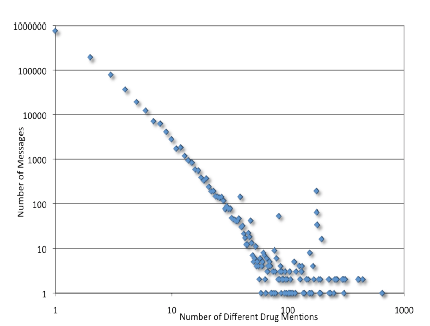
\includegraphics[width=7cm, height=5cm]{Figure-1-Zipfian.png}
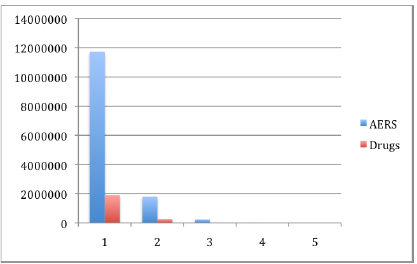
\includegraphics[width=7cm, height=5cm]{Figure-2-AERS_Drugs.png}


The first plot demonstrates a zipfian distribution for drug name mentions in the messags, with more than 96\% of messages mentioning at most 5 drugs, adding confidence to the hypothesis that messages can be associated with at most a handful of drugs. Chee elects to eliminate messages having more than 5 unique drugs as these frequently constitute lists of drugs posted or SPAM messages. The second plot shows that adverse events are mentioned far more often than drug names, suggesting that a preceeding post containing a drug name eliminates referencing it in subsequent posts - much like replies on a forum. Investigating this is an area for future research. Note that the numbers on the X-axis for the 2nd plot refer to the number of terms (1, 2, ...) that comprise the drug name or adverse event - a fact not really relevant for this analysis.

\subsubsection{Handling Multiple Drug Names}
If multiple drugs are mentioned in a single message, it becomes difficult to discern which drug the message should apply to. Another study is conducted to evaluate the typical distance (number of characters) between the top 25 co-occuring drugs in messages to determine if the messages could be segmented into relevant portions for each drug. The analysis shows a Zipfian distribution in the character separation, indicating that most drugs are talked about together within a single sentence, or in adjacent sentences, leading Chee to conclude separation is not possible and that any adverse events mentioned in a message should just be attributed to all drugs mentioned within the message.

\subsubsection{Sentiment Feature}
A final experiment preceeding the main classification work is done to validate how message sentiment will be determined. Chee hypothesizes that the positive or negative valence in a message represents drug satisfaction, making it an interesting feature to incorporate into the classification experiments. A lexicon using the positive emotion, negative emotion, anxiety, anger and sadness terms from LIWC is constructed, augmented to include several emoticons (:), :(, ..) and acronyms (LOl, ROFL, ..). Two case studies are then executed using messages sampled from specific groups in the corpus, and the change in drug sentiment is analyzed over the drug's pre-recall, recall, and post-recall timesframes. This sentiment is compared with a \textif{control} sentiment derived from those messages in the samples not containing the drug to look for a statistically significant difference.

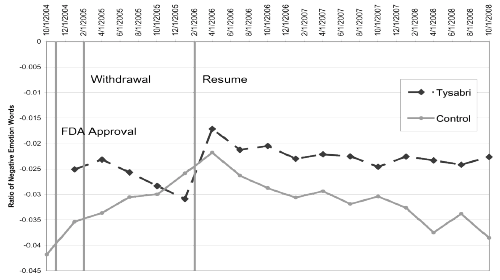
\includegraphics[width=7cm, height=5cm]{Figure-3-Tysabri.png}
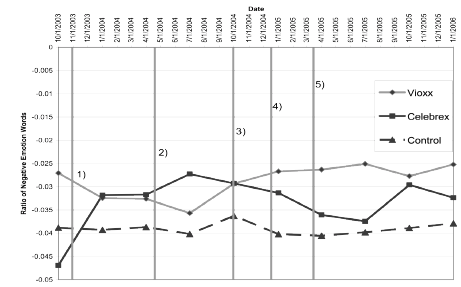
\includegraphics[width=7cm, height=5cm]{Figure-4-Vioxx.png}

The left-most plot shows the sentiment change for Tysabri pre-recall, recall (withdrawal) and post-recall (resume) over the control. It shows a reasonably intuitive change in negative valence to Tysabri having been introduced (more positive), withdrawn (negative), reintroduced (hopeful therefore positive), then stabalizing. The right plot shows sentiment change for a pair of commonly used pain relievers - Vioxx and Celebrex - over the course of several public anouncements and a withdrawal of Viox (sections 1 through 3), then Celebrex (4 and 5). ANOVA is applied to both case studies to determine statistical significance for each drug in each segment against the control. Both were found to be statistically significant with p \< .001.


\subsubsection{Feature Selection, Training and Test Data Size}
The introduction to the main body of classification experiments is preceeded by a brief discussion on the features vectors used, as well as how training, test and validation sets are constructed to support the use of 10-fold Cross Validation for classifier evaluation.

Two types of feature vector are decided upon and then leveraged in the  experiments. The first feature vector type is generated over general vocabulary terms in the messages, selected based on frequency cutoffs. This vector is then augmented with counts from the various specialized lexicons mentioned earlier: medical, diseases, drugs, sentiment and reactions (MedRA). The second feature vector uses only the specialized lexicon.

The richness of the training data is of foremost concern to Chee. There are only 435 drugs having 500 or more unique messages, and only 575 drugs having more than 250 messages, with 63 and 77 watchlist drugs mentioned in each respectively. Therefore approximately 90\% of message instances reference non-watchlist drugs, creating a data scarcity problem when attempting to classify watchlist drugs. Chee decides upon a minimum cutoff of 250 messages per drug for that drug's messages to be included in training and testing. An  experiment is constructed to evaluate techniques to address the scarcity, including scaling features, selecting different ratios of negative to positive training examples such as 1 to 1 and 2 to 1, and experimenting with different split ratios in cross-validation - 90/10 and 80/20. These experiments are dubbed inconclusive and not elaborated on further in the dissertation.

\subsubsection{Classifier and Lexicon Selection}
The next goal of the dissertation's experimentation is to discover the best performing combinations of classifier, lexicons and feature selection as a means to inform the construction of a \textit{meta classifier} to be used in watchlist drug prediction. The inconclusive nature of the data set sizing experiments prompts settling on the following methodology for classifier
training and evaluation:
\begin{itemize}
  \item test and training sets are sampled with the same distribution as the original data. No use of 1 to 1, 2 to 1 or similar negative to positive sample ratios.
  \item Data is divided into a 90/10 split, where 90\% of the samples are used to train and 10\% used to validate
  \item The splits themselves are sampled per the original distribution.
\end{itemize}

The classifier evaluation experiments evaluate combinations of classifier type (Support Vector Machines or Naive Bayes), the optional use of normalization and cost-weighting, and various combinations of the lexicons described earlier. Cost-weighting applies a greater penalty to incorrectly classifying a positive example then a negative one during training, as a means to offset the low prevalence (~13\%) of watchinglist drugs in the training data. The experimental results and analysis make heavy use of acronyms to understand the combinations evaluated:

\begin{center}
  \begin{tabular}{|c|c|}
    \hline
    Acronym & Description\\
    \hline\hline
    UNB & Un-normalized Naive Bayes\\
    \hline
    UNBC & Un-normalized Naive Bayes with Cost Weighting\\
    \hline
    NNB & Normalized Naive Bayes\\
    \hline
    NNBC & Normalized Naive Bayes with Cost Weighting\\
    \hline
    SVM & Un-normalized SVM\\
    \hline
    SVMC & Un-normalized SMV with Cost Weighting\\
    \hline
    NSVM & Normalized SVM\\
    \hline
    dis & disease lexicon\\
    \hline
    react & reactions lexicon\\
    \hline
    drugs & drugs lexicon\\
    \hline
    sent & sentiment lexicon\\
    \hline
    med & medications lexicon\\
    \hline
  \end{tabular}
\end{center}
For example, \textit{drugs\_dis\_sent\_react\_NSVMC} would equate to an experiment using the Normalized SVM with Cost Weighting, incorporating the drugs, disease, sentiment and reaction lexicons.

A series of 240 experiments were run using the combinations above to ascertain the best combination of lexicons to use when evaluated according to accuracy, F1 score, and area under the ROC curve (AUC). Accuracy is reviewed by Chee first, and the top 3 classifier configurations for each accuracy test are presented for context:

\begin{center}
  \begin{tabular}{||c c c c c||}
    \hline
    Experiment Type & Configuration & Accuracy & Lower Bound & Upper Bound \\
    \hline\hline
    CV & \verb|dis_react_NSVM| & 0.903288201 & 0.793206235 & 0.957882075 \\
    \hline
    CV & \verb|drugs_dis_sent_react_NSVM| & 0.901353965 & 0.790801818 & 0.956684149 \\
    \hline
    CV & \verb|drugs_sent_react_NSVM| & 0.901353965 & 0.790801818 & 0.956684149 \\
    \hline
    Test & \verb|drugs_dis_sent_react_UNB| & 0.879310345 & 0.771204077 & 0.940291098 \\
    \hline
    Test & \verb|drugs_sent_react_UNB| & 0.879310345 & 0.771204077 & 0.940291098 \\
    \hline
    Test & \verb|dis_sent_react_UNB| & 0.879310345 & 0.771204077 & 0.940291098 \\
    \hline
    Test(CW) & \verb|drugs_dis_NSVMC| & 0.879310345 & 0.771204077 & 0.940291098 \\
    \hline
    Test(CW) & \verb|drugs_sent_SVMC| & 0.862068966 & 0.750738501 & 0.928415984 \\
    \hline
    Test(CW) & \verb|drugs_sent_NSVMC| & 0.862068966 & 0.750738501 & 0.928415984 \\
    \hline
  \end{tabular}
\end{center}

The accuracy of a naive baseline classifier that labels all instances as negative would be 86.7\% per concentrations of non-watchlist and watchlist drugs in the training data. While several configurations exceed this, when considering 95\% confidence interval defined by the lower and upper bounds there is uncertainty that any classifier is more accurate than the naive baseline. The cost weighting shows no accuracy benefits either.

Discussed next are the F1 and area under the ROC curve (AUC) scores. Analysis of the F1 score also prompts inspection regarding the recall and pecision tradoffs therein, as the F1 score represents a harmonic mean of the two:
\begin{center}
  \begin{tabular}{||c c c||}
    \hline
    Experiment Type & Configuration & F1 Score\\
    \hline\hline
    CV & \verb|drugs_dis_react_NSVM| & 0.476190476 \\
    \hline
    CV & \verb|drugs_dis_react_UNB| & 0.472527473 \\
    \hline
    CV & \verb|drugs_UNB| & 0.4698795518 \\
    \hline
    Test & \verb|drugs_UNB| & 0.470588235 \\
    \hline
    Test & \verb|drugs_dis_UNB| & 0.444444444 \\
    \hline
    Test & \verb|drugs_dis_sent_react_UNB| & 0.363636364 \\
    \hline
    Test(CW) & \verb|drugs_dis_SVMC| & 0.444444444 \\
    \hline
    Test(CW) & \verb|drugs_UNBC| & 0.444444444 \\
    \hline
    Test(CW) & \verb|drugs_react_SVMC| & 0.384615385 \\
    \hline
  \end{tabular}
\end{center}
\begin{center}
  \begin{tabular}{||c c c||}
    \hline Experiment Type & Configuration & AUC \\
    \hline\hline
    CV & \verb|drugs_UNB| & 0.7592 \\
    \hline
    CV & \verb|drugs_dis_UNB| & 0.7564 \\
    \hline
    CV & \verb|med_drugs_NNB| & 0.7545 \\
    \hline
    Test & \verb|dis_UNB| & 0.7514 \\
    \hline
    Test & \verb|drugs_dis_UNB| & 0.6850 \\
    \hline
    Test & \verb|dis_sent_react_UNB| & 0.6675 \\
    \hline
    Test (CW) & \verb|drugs_UNBC| & 0.7825 \\
    \hline
    Test (CW) & \verb|drugs_dis_UNBC| & 0.7075 \\
    \hline
    Test (CW) & \verb|drugs_dis_SVMC| & 0.6900 \\
    \hline
  \end{tabular}
\end{center}

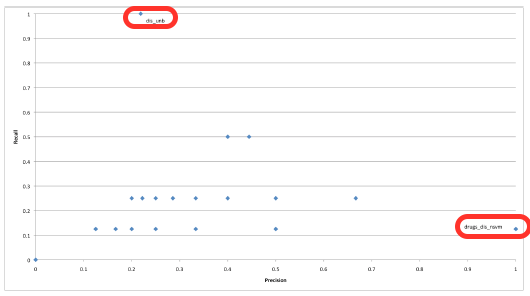
\includegraphics[width=7cm, height=5cm]{Figure-5-F1.png}
The F1 scores are lower where cost-weighting is applied, comparable to accuracy. The image above shows how recall (Y axis) and precision (X) access vary across classifier configurations in the test instance, and a comparable image was seen with cost-weighting: low numbers of high recall or precision outliers, and most of the mass concentrated at low recall and precision. AUC does contain higher scores for cost weighted classifers compared to those non-weighted.

As the goal of this experiment was to identify the value of the lexicons, their prevelance in the top 10 best performing weighted and non-weighted classifiers for each metric is reviewed:
%two tables side by side
\begin{center}
  % caption for non-weighted classifiers
  \begin{tabular}{c c}
    \hline
    Drugs & 33\\
    \hline
    Disease & 32\\
    \hline
    Sentiment & 28\\
    \hline
    Reactions & 27\\
    \hline
    Medical & 7\\
    \hline
  \end{tabular}
  \quad
  % caption for weighted classifiers
  \begin{tabular}{c c}
    \caption{Weighted Classifers}
    \hline
    Drugs & 20\\
    \hline
    Disease & 18\\
    \hline
    Sentiment & 15\\
    \hline
    Reactions & 10\\
    \hline
    Medical & 5\\
    \hline
  \end{tabular}
\end{center}

The ranking favors the drugs, disease and sentiment lexicons, which are then selected for use in the prediction problem. Unfortunately this leads to overfitting concerns because a classifier will learn on the drug names and diseases associated with watchlist drugs. Chee notes disappointment that the reactions lexicon does not rank higher, indicating it may not really capture how people speak about adverse events.

\subsubsection{Evaluating the BNS Lexicon}
Another area of experimental exploration is how the initial word n-gram features are selected to populate the feature vectors. As previously discussed, the top $n-k$ technique is preferred to prompt selection of those word n-grams that are not necessarily the most frequent, but in theory the most informative.

Bi-Normal Separation (BNS) is an alternative technique explored by Chee for discovering those word n-grams. BNS identifies those n-grams that are differentially expressed between two classes: watchlist and non-watchlist messages. BNS lexicons are constructed using the test subset of data for the top 15,000, 10,000 and 5,000 word n-grams, then used in combination with the drugs, diseases and sentiment lexicons, as well as a set of "special features" consisting of numerical counts of:
\begin{itemize}
  \item disease mentions
  \item drug mentions
  \item medical terminology
  \item sentiment containing terms
  \item AERS terminology
\end{itemize}

Experiments were run again using Naive Bayes and SVM classifiers, with optional normalization, optional cost-weighting, and the optional inclusion of the numerical features. The top classifier configuration for each combination of BNS n-grams and numerical features is shown below with its accuracy and confidence bounds:
\begin{center}
  \begin{tabular}{||c c c c c c||}
    \hline
    Configuration & Numericals & BSN & Accuracy & Lower Bound & Upper Bound \\
    \hline\hline
    \verb|bns_drug_dis_sent_NNB| & Yes & All(5k,10k,15k) & 0.8762 & 0.7602 & 0.9405\\
    \hline
    \verb|bns_drugs_dis_sent_NNB| & No & All & 0.8762 & 0.7602 & 0.9405\\
    \hline
    \verb|bns_drugs_dis_sent_NNB| & Yes & (10k, 15k) & 0.8762 & 0.7602 & 0.9405\\
    \hline
    \verb|bns_drugs_dis_sent_NNB| & No & (10k, 15k) & 0.8762 & 0.7602 & 0.9405\\
    \hline
    \verb|bns_drugs_dis_sent_NNB| & Yes & 15k & 0.8762 & 0.7602 & 0.9405\\
    \hline
    \verb|bns_drugs_dis_sent_NNB| & No & 15k & 0.8762 & 0.7602 & 0.9405\\
    \hline
  \end{tabular}
\end{center}

There was no clear advantage to a specific number of BNS features, nor the inclusion of the additional numerical features.  Furthermore, the F1 and AUC scores for this test showed no advantage to a specific BNS or numerical feature combination, though un-normalized Naive Bayes did perform better in F1 and AUC than normalized Naive Bayes as seen above. Regardless, none of the tests showed better accuracy, F1 or AUC than the previous tests using specialized lexicons only. Chee hypothesizes this is in part due to the limited number of messages in the test set BNS could select n-grams from.

\subsubsection{Prediction Watchlist Drugs}
The previous experiments were used to assemble a meta-classifier using the best classifiers based on accuracy, F1 and AUC scores. The following were selected:
\begin{itemize}
  \item Normalized SVM using disease, reaction (AERS) lexicons, having 90.33\% Accuracy
  \item Normalized SVM using drugs, disease and reaction lexicons, having an F1 score of 0.4762
  \item Un-normalized Naive Bayes classifier with an AUC score of 0.7592
\end{itemize}
Two meta-classification experiments are constructed to examine the False Positives produced as an indicator for a possible \textit{future} watchlist drugs if used in an applied setting. The first experiment uses the classifier configurations stated above, but the training data is modified to denote drugs \textit{withdrawn} from the market as non-watchlist. It is important to distinguish that a withdrawn drug would have at one point been a watchlist drug, as drugs are placed on the watchlist - even if briefly - before being removed from the market. By looking for these withdrawn drugs marked non-watchlist in the set of False Positives from the training results, we evaluate the ability to discern new watchlist drugs. This experiment was executed via training runs to build 100 classifiers of each configuration. A scoring methodology is applied using the following linear combination:
\[
  \frac{\#\ of\ False\ Positives}{\#\ of\ Occurrences} * (\#\ of\ False\ Positives) * (\#\ of\ Classifer\ Types)
\]
Each occurence equates to an instance of the withdrawn drug actually being classified in the training. The table below shows the top 5 scores, as well as  those withdrawn drugs identified as false positives.
\begin{center}
  \begin{tabular}{||c c c c c||}
    \hline
    Drug & # Positives & # Occurrences & # Classifiers & Score \\
    \hline\hline
    \textit{clozapine}, Clozaril, FazaClo & 31 & 64 & 3 & 45.047\\
    \hline
    \textit{fludarabine}, Fludara, Oforta & 29 & 61 & 3 & 41.361\\
    \hline
    \textit{methylphenidtate}, Concerta, Daytrana & & & & \\
    Metadate CD, Metadate ER, Methylin & 25 & 50 & 3 & 37.500 \\
    Ritalin, Ritalin LA, Ritalin-SR & & & & \\
    \hline
    \textit{morphine}, Astramorph PF & & & & \\
    Avinza, Duramorph, Infumorph & & & & \\
    Kadian, MS Contin, MSIR & 15 & 38 & 3 & 15.474 \\
    Morphine IR, Oramorph SR, RMS, Roxanol & & & & \\
    \hline
    \textit{meloxicam}, Mobic & 15 & 50 & 3 & 13.500 \\
    \hline\hline
    \textit{thalidomide}, Thalomid & 10 & 36 & 1 & 2.778\\
    \textit{temazepam}, Restoril & 11 & 50 & 1 & 2.420\\
    \textit{hydromorphone}, Diluadid, Dilaudid-HP & & & & \\
    Exalgo, Palladone & 9 & 42 & 1 & 1.929\\
    \textit{trovafloxacin}, Trovan & 9 & 46 & 1 & 1.761\\
    \textit{rofecoxib}, Vioxx & 9 & 50 & 1 & 1.620\\
    \textit{sibutramine}, Meridia & 5 & 27 & 1 & 0.926\\
    \textit{cerivastatin}, Baycol & 1 & 33 & 1 & 0.030\\
    \hline
  \end{tabular}
\end{center}
The generic Sibutramine (Meridia) is of particular interest to this study, as it is under review but not yet an official watchlist drug. FDA has issued safety communications as of November of 2009, and the European Union has removed it from the market.

The second experiment entails removing the withdrawn drugs entirely from training, classifying them after a classifier is built for each fold during cross-validation. This approach is presumed to identify the withdrawn drugs with greater confidence as they are not present in the training data:

\begin{center}
  \begin{tabular}{||c c c c c||}
    \hline
    Drug & # Positives & # Occurrences & # Classifiers & Score \\
    \hline\hline
    \textit{methlyphenidate}, Concerta &   &   &  &  \\
    Daytran, metadate(CD, ER) & 30 & 34 & 3 & 79.412\\
    Methylin(ER), Ritalin(LA,SR) &  &  &  & \\
    \hline
    \textit{morphine}, Astramorph(PF) & & & & \\
    Avinza, Duramorph, Infumorph & & & &\\
    Kadian, MS Contin, MSIR & 13 & 38 & 3 & 13.342\\
    Oramorph SR, RMS, Roxanol & & & &\\
    \hline
    \textit{questiapine}, Seroquel, Seroquel XR & 14 & 31 & 2 & 12.645\\
    \hline
    \textit{indomethacin}, Indocin (IV,SR) & 19 & 37 & 1 & 9.757 \\
    \hline
    \textit{sibutramine}, Meridia & 17 & 34 & 1 & 8.500\\
    \hline\hline
    \textit{trovafloxacin}, Trovan & 33 & 100 & 1 & 10.89\\
    \textit{hydromorphone}, Dilaudid(HP), Exalgo, Palladone & 33 & 100 & 1 & 10.89\\
    \textit{rofecoxib}, Vioxx & 32 & 100 & 1 & 10.24
    \textit{thalidomide}, Thalomid & 10 & 36 & 1 & 2.778\\
    \textit{temazepam}, Restoril & 8 & 28 & 1 & 2.286\\
    \textit{cerivastatin}, Baycol & 2 & 100 & 1 & 0.04\\
  \end{tabular}
\end{center}
Interestingly sibutramine does score significantly higher in this experiment, as do several of the withdrawn drugs (hydromorphone, rofecoxib, trovafloxacin), though Baycol scores much lower.  Additionally, physiciatric drugs (Ritalin) and opiates (morphine) show up near the top in both experiments, presumably because they are more dangerous and more often associated with adverse reactions.


\section{Discussion of Contributions}
The major contribution of the dissertation is a collection of techniques for leveraging public health forum data for pharmacovigilance. Techniques in natural language processing and classification are developed and applied to identify drugs widthdrawn from the market by the FDA by using only the textual features of the messages themselves. The end result was an ensemble classification technique capable of identifying current watchlist drugs - and therefore \textit{future} watchlist drugs.  In the interest of discussion, we can distill this work to X major areas to discuss and critique from the work as its primary contributions:
\begin{itemize}
  \item Exploration and Annotation of Health Forum Data
  \item Techniques for Differentiating Language and Spelling Mistakes
  \item Feature Generation using Speciality Lexicons
  \item Quality of WatchList Predictions
\end{itemize}

\subsection{Exploration and Annotation of Health Forum Data}
Chee's initial exploration of the Yahoo! corpus is informative in its own right, as it exposes the challenges in annotating messages from the general public for use in a scientific study. Scientific documentation - such as medical literature - is usually grammatically correct and highly precise in its use of scientific terminology such as drug names, diseases, side effects. Chee must confront a number of problems, including:
\begin{itemize}
  \item Differentiating between the message content and other artifacts, such as HTML tags, garbage strings, web URLs, and people's names
  \item Colloquial language, abbreviations and slang expressing sentiment, side effects and other medical terminology
  \item Misspellings to critical message content such as medical terminology and drug Names
\end{itemize}

The majority of message tokens contributing to these problems were placed in a general category of \textit{error}, accounting for 4.1\% of each message's tokens on average. This prompts a more in depth exploration into the nature of the errors, discovering that foreign languages appeared to be the largest contributor. However, the methods here did not go much further than identifying that problem tokens were present and attempting to classify them. If the nature of the problem token was known enough to classify them manually, why not replace them with a proper (grammatically correct) token of equivalent meaning, thereby preserving the value of the message? Mondern word processors frequently correcty for mispellings, and slang terminology such as "sux" could easily be replaced by a real world equivalent. Furthermore, these token type statistics were generated against only a 500 message sample of the corpus. It seems this kind of automated analysis could have been extended to encompas all messages in the corpus in order to confirm or deny these patterns.



\subsection{Techniques for Differentiating Language}
Chee had to conduct an in depth analysis of the composition of health forum data to inform his selection of NLP techniques for feature generation. The initial analysis identified a high prevalance of foreign language terms in the messages. This is concerning, as these terms can inflate the word n-gram feature vector size going into the two classification techniques. The training time for an SVM is:
\[
???
\]
Naive Bayes is:
\[
  O(nd), where d = number of features, n = number of samples

\]
It is therefore a worthwhile goal to reduce the classification feature space through the elimination of messages written largely in foreign languages. Chee's approach to eliminating languages that do not use roman (latin) text through Unicode language detection takes immediate advantage of common website text representations in UTF-8, which account for 91.2\% of all websites \citep{UTF-8 article on wikipedia}. As each latin script character is represented by a unique unicode code point (bits - appearing as hexadecimal in text), it is easy to distinguish characters falling outside the range of latin script.

Chee opts for the use of simple, dictionary based methods using lexicons drawn from OpenOffice to classify the individual tokens in a message as english or not for use in an inequality used to score and retain predominantly english messages. Cited is an inability to use other techniques for various reasons:
\begin{itemize}
  \item the common words approach by \citep{Ingle, 1976} is mentioned, but given little attention
  \item n-gram based techniques by Dunning \citep{Dunning} require training data, which he does not have (why not make it?)
  \item n-gram based techniques can skew to repitious words and phrases presents in online forums (e.g. "In Reply to")
  \item Character n-grams can't different between similar languages: Slovenian, Czech, Polish
\end{itemize}

Dunning \citep{Dunning} does give some attention to the common words technique, stating these techniques are suitable when enough text is present to be classified as the common words are often \textit{closed class} words, with examples such as: and, or, this, that. These words often serve a function, such as joining other words and phrases thereby providing structure to the text. Sufficient amounts of text allow this structure to be identified and leveraged in classification. Dunning uses counter examples that are 20-characters long and 3-4 tokens to highlight the limitation, but considering the average 172 token length of the Yahoo! corpus it might have been more informative had Chee explored this technique further.

We could also advocate that Dunning's n-gram language classification technique would have been worth applying to develop a binary english-non-english classifier. Dunning develops his classification technique by modeling languages as a Markov Decision Process, wherein the probability of a particular word or phrase is dependent upon those preceeding it and their probabilities assuming a specific language. Dunning successfully differentiates between english and spanish texts of small length: 10, 20, 50, 100 and 200 bytes, having used relatively small training texts between 1000 and 50000 bytes. It seems reasonable that small sampling of longer, english only messages could have been identified as a training set to leverage this technique.

Additionally, recall the inequality $(4 * foreign) + unknown + ignore > english + drugs + medical$ used in message classification. Little beyond the initial token counts by type indicating foreign language prevalance and the resulting ~18.7\% reduction in message count thanks to the technique is provided as evidence of effectiveness. Chee himself noted that tokens can be part of multiple languages, yet the algorithm for counting tokens always favored english, likely skewing the counts:
\[
if ((word) in Ingore list) OR (word length < 2) OR (word contains "@"), ignore count ++
Else if (word in English list)
English Count++
.....
\]
The vocabulary of the english language has been highly influenced by french and germanic languages \citep{Wikipedia page for english}, accounting for more than 55\%. This approach seems vulnerable to misclassification.

Finally, one would expect meta-data in the Yahoo! corpus messages might help discern the locality of the writer. Consider properties such as the name of the forum a message is under being english or not, or an IP address associated with a user being geo-resolvable to a US location.

While language classification is cited as a contribution of the dissertaton, the utility and accuracy of this approach is questionable.


\subsection{Named Entity Recognition: Drugs and Drug Effects}
Chee again favors dictionary methods for identifying drugs and drug effects within messages. The drug effects lexicon is composed from the FDA Adverse Event Reporting System (AERS), which uses the Medical Dictionary for Regulatory Activities (MedDRA) when coding reactions in the reports \citep{FAERS}. MedDRA has an onotological structure characterized by a top-most level of "System Organ Classes" (SOCs), two intermediate levels of high-level terms (term groups and terms themselves) falling within a SOC, followed in the the lowest levels by a preferred term (PT) and its synonyms, lowest level terms (LLT). It is the LLT or PT that may be recorded in a AERS report. Preferred terms are typically clinically correct, with the LLT being a more relaxed, colloquial phrase:
\begin{itemize}
  \item Nausea,  Feeling queasy
  \item Influenza,  Flu
\end{itemize}

The number of AERS (MedDRA) term instances found across the lucene indexed corpus of ~10M messages was 13,794,445. The experimental results published by Chee (Figure 13 in the dissertation) do show at least 1 AERS hit per message, indicating this approach worked and may be viable for recognizing adverse reactions in online, english text.

The results for drug identification were less promising.  The drug lexicon was composed from the FDA and a drugs taxonomy on Drugs.com. Chee outright states limitations in this approach as it does not account for all therapeutic biologicals, foreign names of drugs, nor the names of drugs not approved for US use. The volume of drug mentions was considerably less than the total number of messages, at 2,228,588. Several challenges make it difficult to discern the presence of a drug in a message:
\begin{itemize}
  \item limitations of the lexicon
  \item some drugs having brand names that are common words (e.g. Commit, used for curbing smoking habits)
  \item slang or colloquial terms
\end{itemize}

Without a broader lexicon, it is difficult to claim this method is successful at identifying drugs in messages. Low volume of drug identification in messages is one of the chief limitations of the work, in that very few watchlist drugs (77) were found, restricting the volume of training data.

Finally, the dictionary based approach looks only for the presence of a token in a message. It does not leverage the value that Part-of-Speech (POS) tagging could provide by differentiating between nouns (drugs), verbs, adverbs and other word categories.


\subsection{Feature Generation using BNS, Speciality Lexicons}
The Bi-Normal Separation (BNS) lexicon experimentation was intended to determine if word features (n-grams) expressed differently between watchlist and non-watchlist messages could serve as useful features in differentiating between the two classes. A study by Forman \citep{Forman} showed strong preference to BNS for feature in text classification for its ability to deduce word features occuring with greater prevalence in one class vs. another. Unfortunately the BNS experiments actually showed worse results compared to the use of the specialized lexicons by themselves. There were some methodological issues in the testing worth discussing:
\begin{itemize}
  \item the BNS lexicons were constructed using the test subset of the data, representing only 10\% of the Messages
  \item each BNS lexicon (5k, 10k, 15k) was tested in conjunction with the other speciality lexicons
\end{itemize}

The former was intentional to avoid biasing the classifier to just the Yahoo! corpus, but at the same time may have contributed to the poor performance of the classification experiments relative to non-BNS tests due to the reduced sample size. The inclusion of the speciality lexicons appears to have been done because this test followed the initial testing on the speciality lexicons only. At no point do we get to see the BNS selected n-grams in isolation.

The sentiment lexicon was another disappointment. While isolated evaluation with certain drugs (Tysabri, Vioxx) showed some changes in sentiment relative to a drug's watchlist status, sentiment did aid in greatly distinguishing messages as pertaining to watchlist or non-watchlist drugs. Chee hypothesizes this is because drug sentiment could be positive for drugs treating difficult illness despite significant side effects.

The drug and disease lexicons provide the best classifier performance. This is concerning because it could cause a classifier to overfit to drug names, hindering its ability to predict new watchlist drugs. Overall, the disertation seems to have been unsuccessful in finding a clear set of word features to separate watchlist from non-watchlist drugs.



\subsection{Quality of Watchlist Predictions}
Initially one would not be satisified with the minimial difference in accuracy shown between a naive classifier classifying each drug as non-watchlist (86\%) versus the accuracy observed in some of the best trained SVMs (90\%). Furthermore, the F1 and AUC scores were that exciting either. However, consider how these scores are defined:
\[
  Accuracy = \frac{TP + TN}{TP + TN + FP + FN}
\]
\[
  F1 = 2 \cdot \frac{precision * recall}{precision + recall}, \ precision = \frac{TP}{TP+FP},\ recall = \frac{TP}{TP+FN}
\]
\[
  AUC = P(X_{1} > X_{0}),\ X_{1} = \verb|Classifier Score of randomly chosen positive instance|,\ X_{0} = \verb|Classifier Score of randomly chosen negative instance|

  is the classifier score of a randomly chosen positive instance, and X_{0} the score of a randomly chosen negative instance. AUC = 1 is perfect classification, where positives instances are always classified higher than negative.
\]
TP, TN, FP, FN stand for true positive, true negative, false positive and false negative respectively. A naive classifier assuming all instances were negative (non-watchlist) would have AUC and F1 scores of 0 and contribute nothing towards the goal of discovering future watchlist drugs. Additionally, note that each performance metric places value on the distinction between a true positive and a false positive, yet false positives are the means by which the value of the approach is communicated.  While it is counterintuitive to say a false positive result is diserable, the detection of a future watchlist drug via this technique would be represented as a false positive. Drugs do not become watchlist drugs until labeled so by the FDA. It might have been interesting had Chee presented and experiment those classifiers having the highest \textit{recall} rates though as observed, these frequently had very low precision would likely have contributed significant numbers of false positives that are just noise - drugs not bound for the FDA watchlist.

Chee's technique was successful in identifying a number of drugs withdrawn from the market despite their having been labeled as non-watchlist:  Palladone,  Trovan, Vioxx, and Baycol. Futhermore, the discovery of \textit{Sibutramine} (Meridia) was compelling because the time frame of the data set used stopped one year before Meridia was placed on a watchlist, demonstrating the ability to detect future watchlist drugs. It is far better to accidentally label a drug as a false positive, watchlist candidate than mistakenly mark it as false negative, failing to call attention to it and allowing considerable, sometimes deadly health consequences to go unnoticed.

The technique in this dissertation is not perfect by any means, but the approach developed does hold value as an augmentation to existing pharmacovigilance programs and techniques. The FDA AERS program is highly dependent on required reports filed by drug manufacturers and voluntary reports form health care providers, patients and their stakeholders \citep{FDA Aers}, and can in no way characterize the true incidence rate of adverse events in the U.S. population. Public health forums represent an interesting data source given how people are more likely to disclose health issues in a comfortable, social setting with peers, and the low barrier of entry for contributing to these conversations.


\section{Techniques and Algorithms}

Discuss:
   - KL divergence
   - SVMs
   - Naive Bayes
  - Cost Weighting and Normalization

\subsection{KL Divergence}




\subsection{Bi-Normal Separation}


\subsection{Support Vector Machines}
SVMs map features into a high-dimensional space using a kernel function \citep{Cortes and Vapnik}.
A hyperplane is constructed that defines the decision boundary between two classes
in this decision space, with those new observations being classified based on which
side of the hyperplane they fall on. Chee quotes studies by Forman & Joachims stating
SVM's strengths in text classification, justifying its use in comparison to Naive
Bayes.
- LibSVM was used with a radial basis function (RFB) kernel
- SVM solves the following optimization problem
\[
  min_{u, b, \xi} \frac{1}{2}w^{T}w + C \sum_{i=1}^{l}\xi i \\
\]
\[
  y_{i}(w^{T}\phi(x_{i}) + b) \gte 1 - \xi_{i}
\]
\[
  \xi_{i} \gte 0
\]

- RBF's are non-linear in nature which gave some accuracy advantages over linear
- RBF's are trained on two parameters $C$ and $\gamma$
- Grid search method using cross-validation is employed to look for $C$ and $gamma$
because it parallelizes well
- $C$ is the penalty parameter for the error term
- RBF kernel is defined as $K(x_i, x_j) = exp(-\gamma||x_i - x_j||^{2}), \gamma > 0$

\subsection{Naive Bayes Classification}
The dissertation uses Naive Bayes classification to address the NLP problems
faced by Chee.  Their use was somewhat counterintuitive because Naive Bayes
Classifiers assume independence of features (words), whereas we know in real world settings
that if a word like "aspirin" were present, there is a greater probability of the
the words "headache" or "pain" being present than "lemonade". However, in
applied settings they still do reasonably well \citep{Manning, 1999}. NB has done well
in SPAM detection \citep{Sahami} and make sense as a first step for their simplicity (no
hyperparameters).

- given word grams $w$ in messages about a drug $D$
- $p(w_{i}|C)$ probability the $i-th$ word is from class C, C is watchlist or
non-watchlist drugs.
- $p(D|C) = \prod p(w_{i}|C)$ - probability of a given drug given the class
- W = watchlist, so $P(D|W) = \prod p(w_{i}|W)$.
- Bayes rule writes this as
\[
  p(W|D) = \frac{p(W)}{p{D}} \prod p(w_{i}|W)
\]
\[
  p(\neg{W}|D) = \frac{p(\neg{W})}{p(D)} \prod p(w_{i}|\neg{W})
\]

Chee combines these two probability modles with the maximum a posteriori (MAP)
decision rule to pick the most likely hypothesis.
<discuss maximum a posteriori method>
- The method of MAP then estimates $\theta$ as the mode of the posterior
distribution of this random variable


\section{Literature Review}
What else is out there that is relevant in this space?  Other studies
that have used public data for medical purposes?



\section{Application Areas}
The most likely area is drug safety surveillance in uncontrolled settings.

- could we also use this in discovering underlying conditions?
- drug combinations?
- confounding fator disccovery??
Write up 1 to 2 pages here.


\section{Concluding Remarks}
Conclude the critique with a few endcap statements about what I learned from it,
where it could go, how it could motivate future research, etc.


\section{Paper Criteria (Grading)}
The critique should include a summary of the research reported, a discussion of the major contributions
claimed, and an assessment of the significance of those contributions and of the research itself. The
critique should also include a brief literature review of the topic related to the thesis, discussion of relevant
algorithms, and application areas for the research reported.

Where appropriate, the critique should
include a comparison with other issues discussed in class. Students are encouraged to select a
dissertation that is related to their course projects.
The evaluation criteria for the critique are as follows:
• Overview of the research reported (20%)
• Review of the related literature (15%)
• Major contributions of the thesis (20%)
• Understanding of techniques and algorithms (20%)
• Application areas (15%)
• Proper construction and readability of paper (10%)




\newpage



\subsection{Feature Selection}
- BNS (Bi-Normal Separation) cited by \citep{Forman}
outperforms other methods for rating & ranking feature importance for Classification

- IG (Information Gain)
Best practice suggested words occuring less than 3 times in a data set should be removed

\subsection{Evaluation Metrics Used}
- watchlist drugs are the positive examples
- non-watchlist drugs are the negative examples
- watchlist drugs that are false positive are the interesting ones from Classification
- had to work with a 90/10 split where 90\% of instances are one class (non-watchlist) and 10\% are another
(watchlist) it is difficult to outperform a naive classifier that just marks everything as non-watchlist
- Receiver Operating Characterisitcs (ROC) curves are used with their Area Under the Curve (AUC)
evaluated.
- ROC curves are the true positive




\subsection{Citations}
https://www.fda.gov/Drugs/GuidanceComplianceRegulatoryInformation/Surveillance/AdverseDrugEffects/


Ingle, Norman. (1976). A language identification table.
The Incorporated Linguist, 15(4):98:101.

Dunning, T. (1994). Statistical identification of language. Technical report, Computing
Research Lab - New Mexico State University.


Dunning, T. (1994). Statistical Identification of Language. Computing Research Laboratory,
New Mexico State University.

HTML language specification: https://www.w3.org/TR/html4/

MedDRA heirarchy:  https://www.meddra.org/how-to-use/basics/hierarchy

FAERS: https://www.fda.gov/drugs/guidancecomplianceregulatoryinformation/surveillance/adversedrugeffects/ucm2007060.htm

BNS:
G. Forman. An extensive empirical study of feature selection
metrics for text classification. J. Mach. Learn. Res., 3:1289–
1305, 2003


\vskip 0.2in
\bibliography{sample}

\end{document}
